\section{Rancangan Sistem Tiket}

\subsection{Komponen Sistem Tiket (tanpa Pengendalian Aliran)}

Komponen sistem tiket dapat dibagi menjadi beberapa bagian, yaitu layanan tiket, basis data relasional, dan kluster Redis. Komponen basis data relasional dapat dibagi menjadi tiga jenis, yaitu kluster PostgreSQL dengan replika baca, kluster CitusData, dan kluster YugabyteDB. Komponen ini yang akan menjadi sumber kebenaran utama dari sistem ini. Selain itu, kluster Redis digunakan untuk menyimpan data agregat ketersediaan berdasarkan area. Arsitektur ini diilustrasikan pada Gambar \ref{fig:ticket-nofc}.

\begin{figure}[htbp]
    \centering
    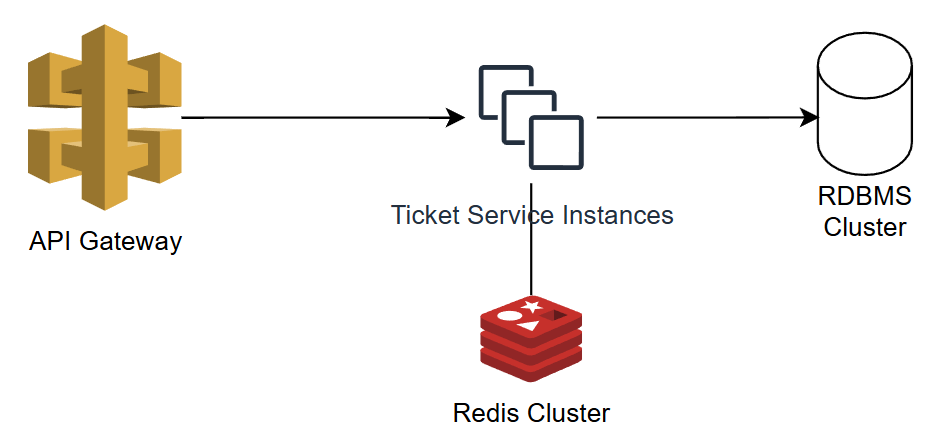
\includegraphics[width=0.8\textwidth]{resources/chapter-3/ticket-nofc.png}
    \caption{Diagram Arsitektur Sistem Tiket Tanpa Pengendalian Aliran}
    \label{fig:ticket-nofc}
\end{figure}

\pagebreak

\subsection{Komponen Sistem Tiket (dengan Pengendalian Aliran)}

Pada sistem tiket dengan pengendalian aliran, terdapat dua komponen baru yaitu RabbitMQ dan pemroses pesanan. RabbitMQ bertugas untuk menyimpan antrean permintaan pemesanan tiket dan pemroses pesanan bertugas untuk memproses pemesanan tiket. Selain itu, kluster Redis memiliki tanggung jawab tambahan untuk menyimpan data yang digunakan untuk menolak permintaan pesanan yang masuk lebih awal. Arsitektur ini diilustrasikan pada Gambar \ref{fig:ticket-fc}.

\begin{figure}[htbp]
    \centering
    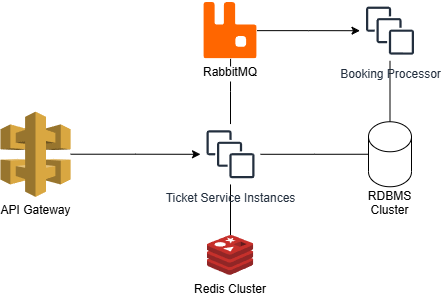
\includegraphics[width=0.8\textwidth]{resources/chapter-3/ticket-fc.png}
    \caption{Diagram Arsitektur Sistem Tiket dengan Pengendalian Aliran}
    \label{fig:ticket-fc}
\end{figure}

\subsection{Variasi Basis Data Relasional}

Gambar \ref{fig:rdbms-variation} mengilustrasikan variasi pengaturan basis data relasional yang mungkin terjadi.

\begin{figure}[htbp]
    \centering
    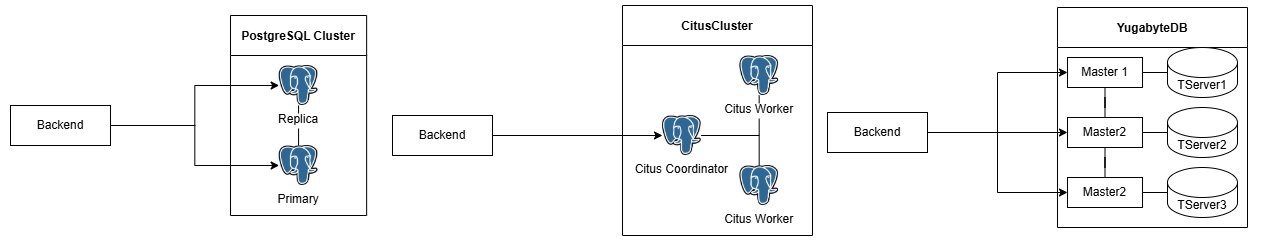
\includegraphics[width=1\textwidth]{resources/chapter-3/rdbms.png}
    \caption{Variasi Basis Data Relasional}
    \label{fig:rdbms-variation}
\end{figure}

Pada konfigurasi kluster PostgreSQL, klien terhubung dengan semua instans. Pada konfigurasi CitusData, klien hanya terhubung dengan koordinator dan koordinator yang akan meneruskan permintaan kepada \textit{worker}. Pada konfigurasi YugabyteDB, klien terhubung dengan semua Master yang masing-masing terhubung dengan TServer. Klien sebenarnya dapat terhubung dengan salah satu master saja, tetapi konfigurasi seperti ini membuat koneksi klien ke YugabyteDB menjadi lebih tahan terhadap kegagalan dan juga dapat mengurangi beban agar tidak terpusat pada satu instans saja.

Konfigurasi kluster PostgreSQL memiliki skalabilitas yang terbatas dengan peningkatan penulisan hanya dapat dicapai dengan penskalaan secara vertikal. Laju penulisan CitusData dan YugabyteDB dapat ditingkatkan dengan menambah jumlah instans.

\textit{Pooler} PGCat akan digunakan agar direct connection basis data yang terbatas dapat digunakan ulang dan dipakai oleh client yang lebih banyak. Selain itu, pada konfigurasi kluster PostgreSQL \textit{pooler} ini berguna sebagai pembagi beban kueri baca antara \textit{primary} dan replika.

\subsection{Integrasi Layanan Pembayaran}

Sistem tiket terintegrasi dengan layanan pembayaran yang disimulasikan (\textit{mock service}). Rancangan layanan ini dibahas pada Lampiran ref{apx:payment-service}.

\subsection{Alur Sistem Tiket}

\subsubsection{Alur Fitur Acara}

Terdapat tiga operasi pada fitur acara, yaitu membaca ketersediaan acara, membaca agregat ketersediaan area, dan membaca ketersediaan kursi. Operasi baca agregat ketersediaan area menggunakan data agregat yang dipelihara pada Redis alih-alih melakukan agregat dari basis data. Operasi baca ketersediaan kursi membaca langsung data dari basis data dengan sedikit pengoptimalan dengan menggunakan tembolok mikro. Alur fitur ini diilustrasikan pada Gambar \ref{fig:flow-event}.

\begin{figure}[h]
    \centering
    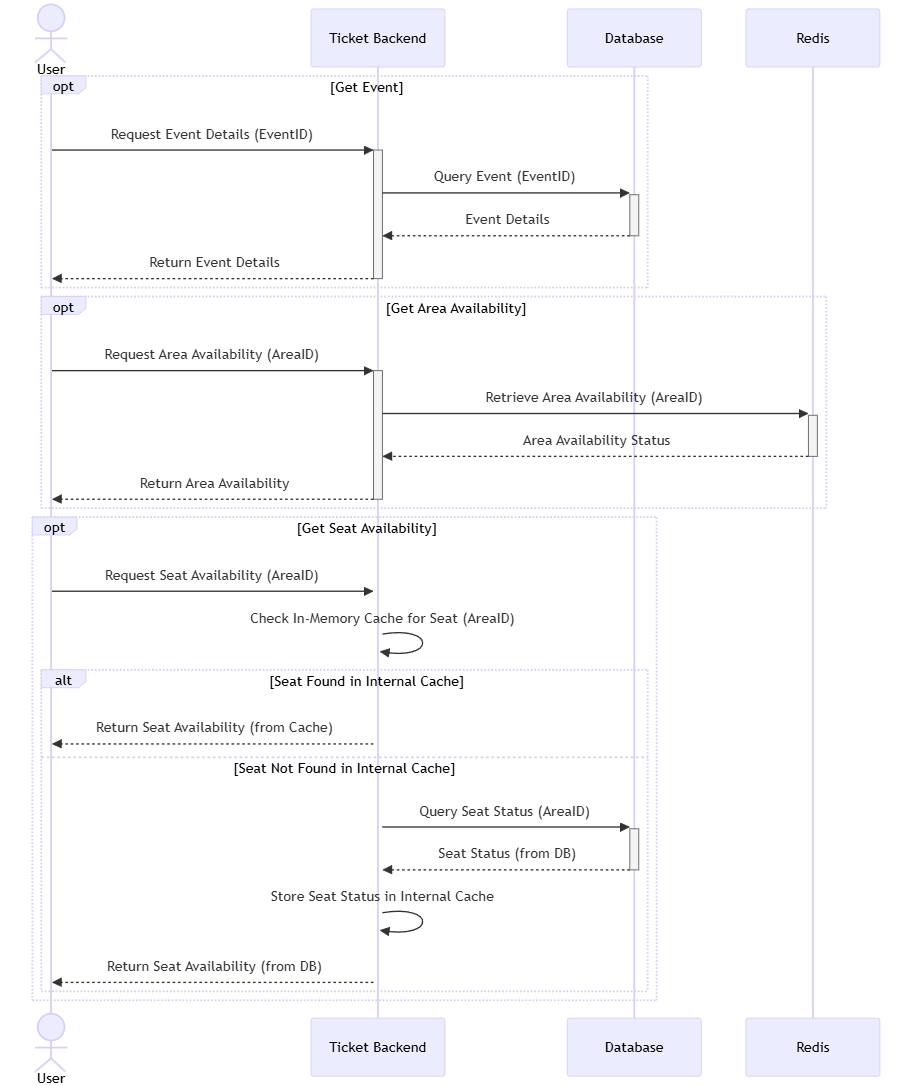
\includegraphics[width=1\textwidth]{resources/chapter-3/event-flow.png}
    \caption{Diagram Alur Fitur acara}
    \label{fig:flow-event}
\end{figure}

\pagebreak

\subsubsection{Alur Fitur Pemesanan Tiket (tanpa pengendalian aliran)}

Proses pemesanan tiket dimulai dengan pengguna mengirimkan permintaan pemesanan kepada sistem tiket. Alur fitur ini diilustrasikan pada Gambar \ref{fig:flow-book-flow}.

\begin{figure}[htbp]
    \centering
    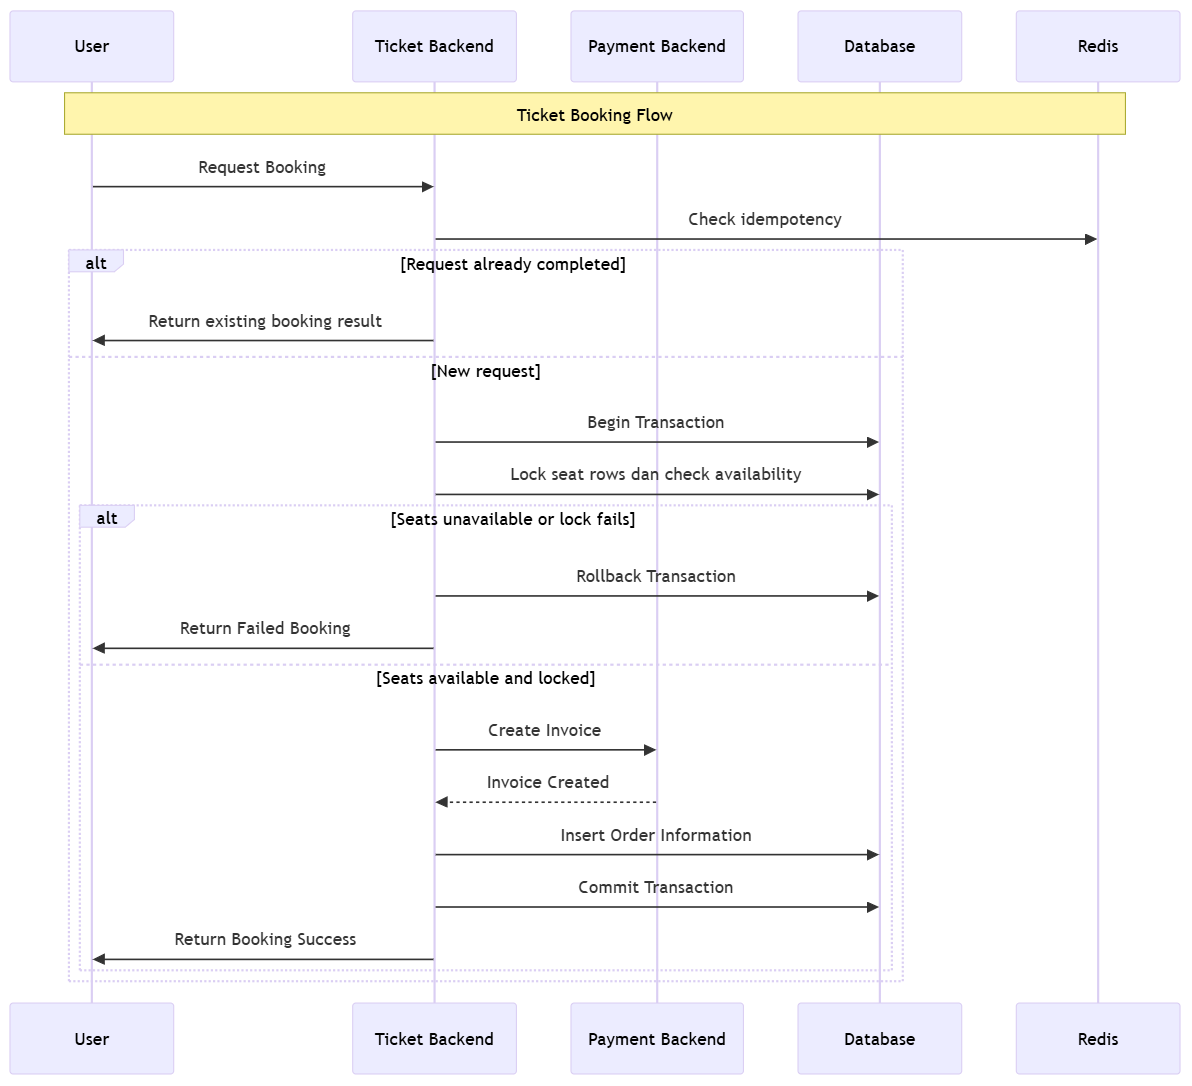
\includegraphics[width=1\textwidth]{resources/chapter-3/book-flow.png}
    \caption{Diagram Alur Fitur Pemesanan Tiket (tanpa pengendalian aliran)}
    \label{fig:flow-book-flow}
\end{figure}

\pagebreak

Ketika pengguna berhasil memesan, pengguna akan melakukan pembayaran kepada gerbang pembayaran. Setelah pembayaran selesai, pengguna memeriksa status pesanan yang telah dibuat. Alur fitur ini diilustrasikan pada Gambar \ref{fig:flow-order-payment-flow}.

\begin{figure}[h]
    \centering
    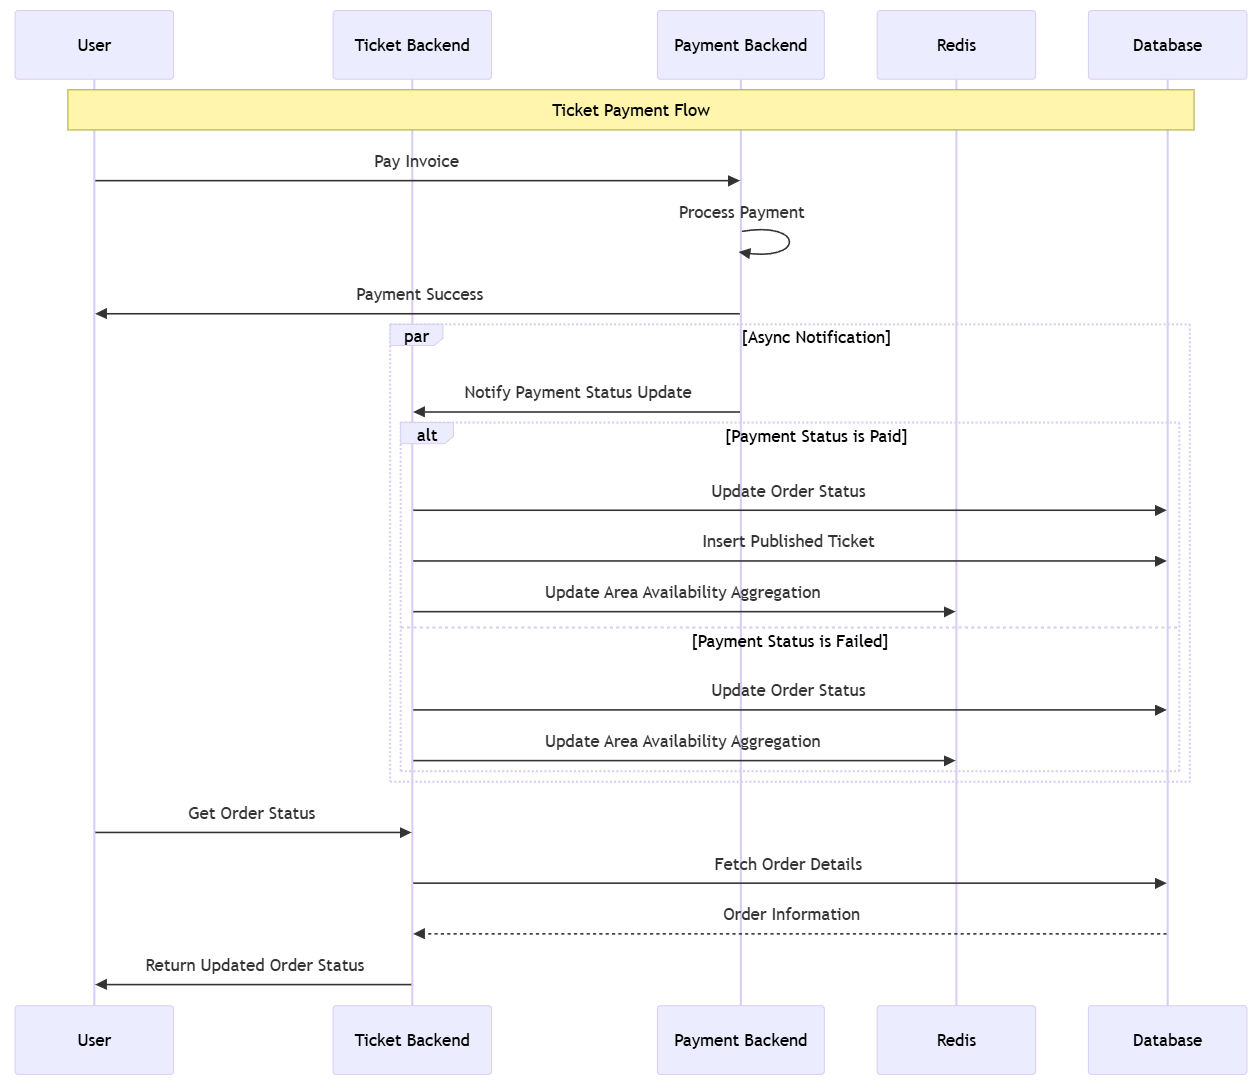
\includegraphics[width=1\textwidth]{resources/chapter-3/order-payment.png}
    \caption{Diagram Alur Fitur Pembayaran Tiket (tanpa pengendalian aliran)}
    \label{fig:flow-order-payment-flow}
\end{figure}

\pagebreak

\subsubsection{Alur Fitur Pemesanan Tiket (dengan pengendalian aliran)}

Proses pemesanan tiket dimulai dengan pengguna mengirimkan permintaan pemesanan kepada sistem tiket. Perbedaan dengan alur tanpa pengendalian aliran adalah penggunaan RabbitMQ dan pemroses pesanan. Proses pemesanan akan diproses secara \textit{partial synchrony} agar sistem dapat memproses pesanan sesuai dengan kapatiasnya. Selain itu, pendekatan ini juga memeriksa data dari Redis untuk menolak sebuah pesanan ketika terdapat pesanan yang sama untuk suatu kursi, tetapi memiliki pesanan lain yang sedang diproses dan belum sepenuhnya berhasil. Alur fitur ini diilustrasikan pada Gambar \ref{fig:flow-book-fc}.

\begin{figure}[h]
    \centering
    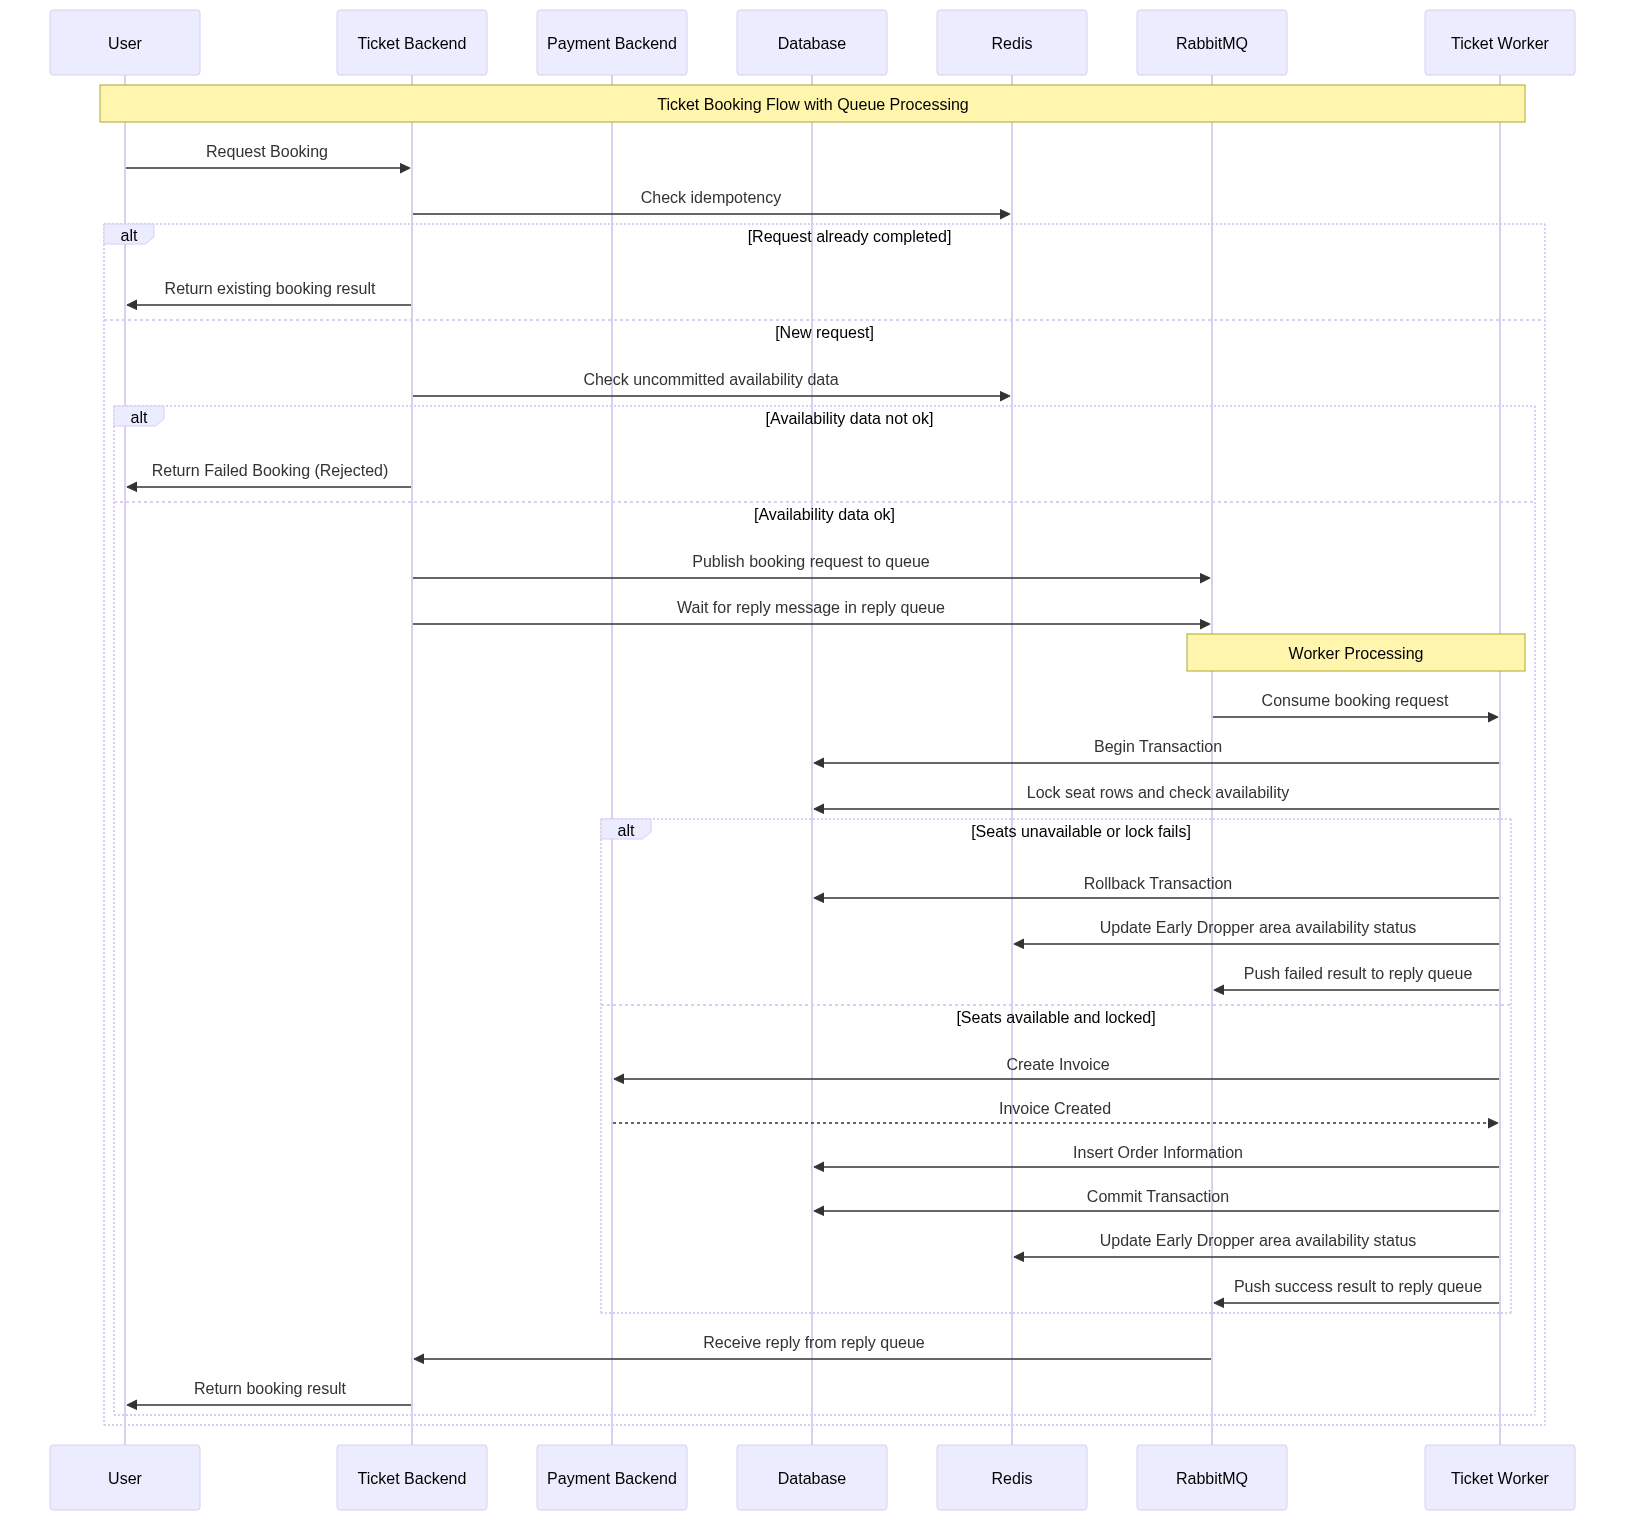
\includegraphics[width=1\textwidth]{resources/chapter-3/book-async.png}
    \caption{Diagram Alur Fitur Pemesanan Tiket (dengan pengendalian aliran)}
    \label{fig:flow-book-fc}
\end{figure}

\pagebreak

Ketika pengguna berhasil memesan, pengguna akan melakukan pembayaran kepada gerbang pembayaran. Setelah pembayaran selesai, pengguna memeriksa status pesanan yang telah dibuat. Tidak ada perbedaan signifikan selain pembaruan data pada Redis untuk sinkronisasi data yang menjadi basis untuk menolak permintaan pesanan lebih awal. Alur fitur ini diilustrasikan pada Gambar \ref{fig:flow-order-payment-fc}.

\begin{figure}[h]
    \centering
    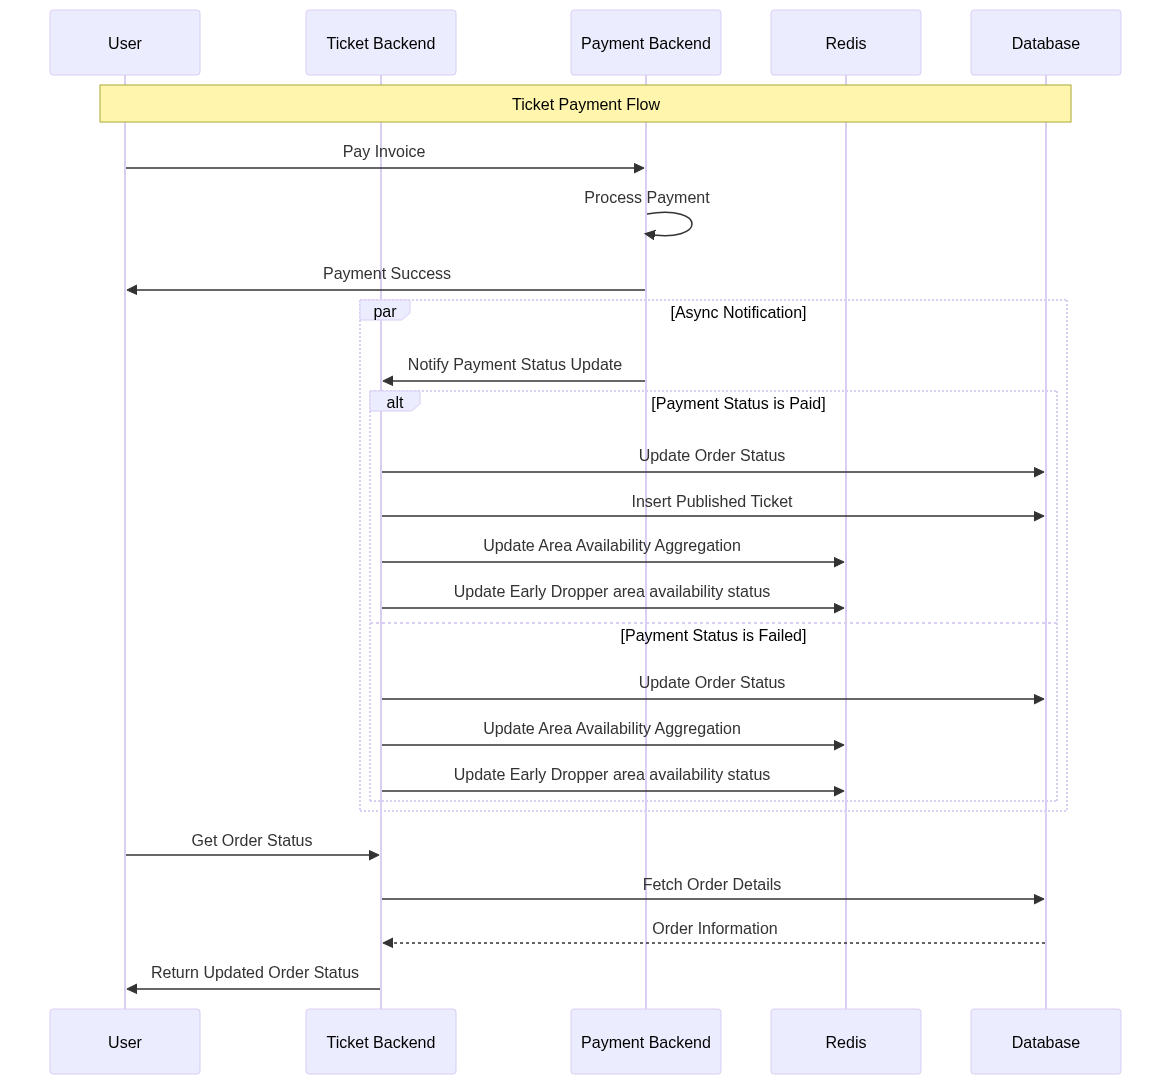
\includegraphics[width=1\textwidth]{resources/chapter-3/order-payment-fc.png}
    \caption{Diagram Alur Fitur Pembayaran Tiket (dengan pengendalian aliran)}
    \label{fig:flow-order-payment-fc}
\end{figure}

\pagebreak

\subsubsection{Alur Fitur Pembacaan Pesanan}

Terdapat dua operasi tambahan yang berkaitan dengan pembacaan pesanan, yaitu membaca detail pesanan dan membaca tiket yang sudah diterbitkan. Alur fitur ini diilustrasikan pada Gambar \ref{fig:flow-order-flow}.

\begin{figure}[h]
    \centering
    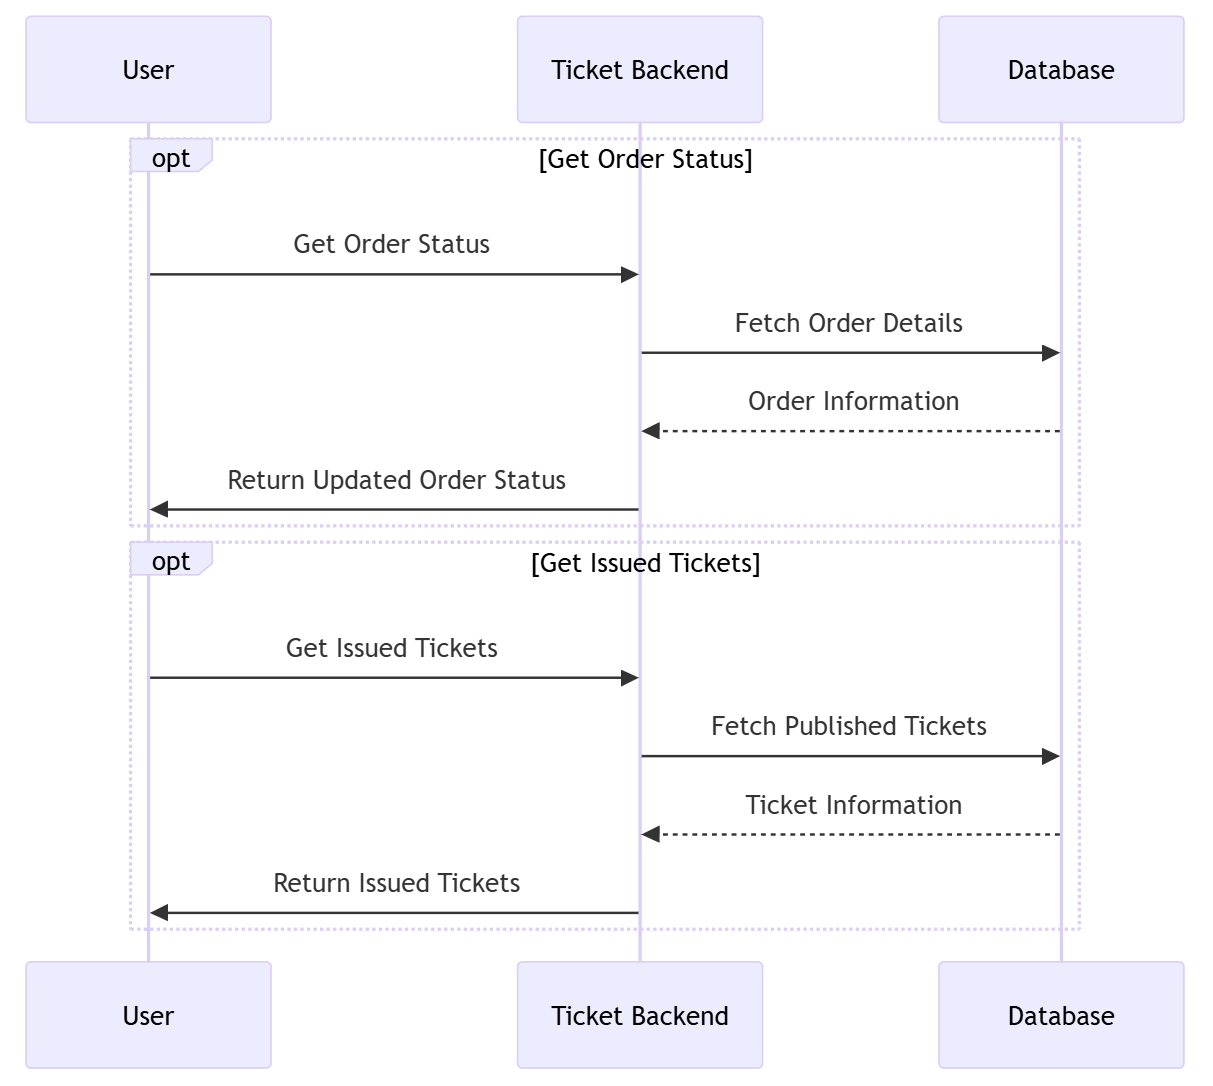
\includegraphics[width=1\textwidth]{resources/chapter-3/order-flow.png}
    \caption{Diagram Alur Fitur Pembacaan Pesanan}
    \label{fig:flow-order-flow}
\end{figure}